\chapter{Analysis of the results}\label{chap:chap5}

This chapter contains a discussion of the results of the platform evaluation, as well as the program that was firstly shown and the program that ended up being developed.\newline

\section{Testing}

Effective backend testing is crucial for ensuring the reliability, functionality and security of the Dharma Network project.\newline

During the development of this project, the approaches used for backend testing in the Dharma Network were manual testing and unit testing. By examining the benefits and limitations of each approach, we can assess their effectiveness in ensuring the quality of the backend components.\newline

\subsection{Manual Tests}
Manual testing involves the systematic execution of test cases by human testers to validate the behavior and functionality of the backend system. In the context of the Dharma Network, manual testing plays a significant role in uncovering potential issues, verifying system responses and evaluating the overall user experience.\newline
\begin{comment}
    Some of the \textbf{benefits of Manual Testing} are:

\begin{itemize}
    \item \textit{Flexibility:} Manual testing allows testers to adapt and explore different test scenarios based on their knowledge and intuition. It enables the identification of edge cases and unexpected behaviors that may not be covered by automated tests.
    \item \textit{User Perspective:} Manual testing provides testers with an opportunity to evaluate the system from the perspective of end-users. It helps in validating the user interface, user interactions, and the overall usability of the backend system.
    \item \textit{Comprehensive Validation:} Manual testing enables testers to perform a comprehensive assessment of various functional and non-functional aspects, such as data validation, error handling, security vulnerabilities, and performance under real-world conditions.
\end{itemize}

However, some limitations of Manual Testing are:

\begin{itemize}
    \item \textit{Time-Consuming:} Manual testing can be time-consuming, especially when the system has a large codebase or frequent updates. Each test case needs to be executed manually, which may limit the number of tests that can be performed within a given timeframe.
    \item \textit{Human Error:} Manual testing is susceptible to human error. Testers may overlook certain scenarios or make mistakes during test execution, potentially leading to undetected issues or false results.
    \item \textit{Limited Test Coverage:} Due to time constraints and the human factor, it may not be possible to cover all possible test scenarios manually. This can result in gaps in test coverage and leave certain parts of the backend system untested.
\end{itemize}
\end{comment}

\subsection{Unit Tests}
Unit testing involves the creation of automated tests for individual units or components of the backend system. In the context of the Dharma Network, unit tests focus on verifying the behavior and correctness of specific functions, methods or classes.\newline
\begin{comment}
    Benefits of Unit Tests:

\begin{itemize}
    \item \textit{Automation:} Unit tests can be automated, allowing for faster and more frequent execution compared to manual testing. This enables developers to catch regressions early and maintain the stability of the backend system.
    \item \textit{Targeted Testing:} Unit tests provide targeted testing at the granular level, allowing for the identification of specific issues within isolated components. This helps in isolating and debugging problems, leading to more efficient troubleshooting.
    \item \textit{Test Coverage:} Unit tests facilitate higher test coverage by systematically examining individual components. Developers can create multiple test cases to cover various scenarios, ensuring a thorough examination of the backend system.
\end{itemize}

Limitations of Unit Tests:

\begin{itemize}
    \item \textit{Limited Scope:} Unit tests focus on individual units or components, meaning that they may not capture the interactions and dependencies between different parts of the backend system. Integration testing is required to validate the interactions and collaborations between these units.
    \item \textit{Incomplete System Validation:} Unit tests alone cannot provide a complete validation of the entire backend system. While they ensure the correctness of individual units, they may not uncover issues that arise from the integration of these units.
\end{itemize}
\end{comment}

To ensure a robust backend, a combination of manual testing and unit tests is recommended. Manual testing can focus on user experience, while unit tests can ensure the correctness and stability of individual components. The synergy between manual testing and unit tests contribute to the overall quality and success of the Dharma Network project.\newline

Here's an example of some of the tests performed:

\textbf{Test 1:}
\begin{enumerate}
    \item Leave empty values on the environment variables to see if they used the default ones
\end{enumerate}

\textbf{Test 2:}
\begin{enumerate}
    \item Introduce the default variables
    \item Introduce the information to retrieve- \texttt{commits}
    \item Compare retrieved information with information displayed on GitHub
\end{enumerate}

\textbf{Test 3:}
\begin{enumerate}
    \item Introduce the default variables
    \item Introduce the information to retrieve- reviews
    \item Compare retrieved information with the reviews on GitHub, keeping in mind the definition of review seen on section \ref{review}
\end{enumerate}

\textbf{Test 4:}
\begin{enumerate}
    \item Introduce the default variables
    \item Introduce the information to retrieve
    \item That information will have some empty fields, such as \texttt{user}, so it retrieves the information related to the entire team on that \texttt{since} date
    \item Compare retrieved information with the information on GitHub
\end{enumerate}

\section{Analysis of the project}

To begin the analysis, it is essential to understand the project's objectives. These objectives serve as the guiding principles that shape the project's direction and determine its success.\newline

As far as the objectives for this project, they have changed throughout the time.

\subsection{Initial vs. Final Sprint Distribution}\label{sprint}

The Sprint Distribution was one of the first things discussed, presented as pioneer plan by the company, during the first meeting, on January 11th 2023. On this meeting, Bruna and Emanuel dialogued about the languages and frameworks necessary for the project, as well as needed hardware, such as the MacBook Pro utilized during its development.\newline

A few weeks later, when the institutional protocols were signed and the internship was ready to start,  the first planning and distribution was presented (see figure \ref{sup_sch}).\newline

A Google Docs file with the entire period  and activities of the internship distributed by weeks was presented (see figure \ref{sup_days}).\newline

 \begin{figure}[htbp]
	\centering
	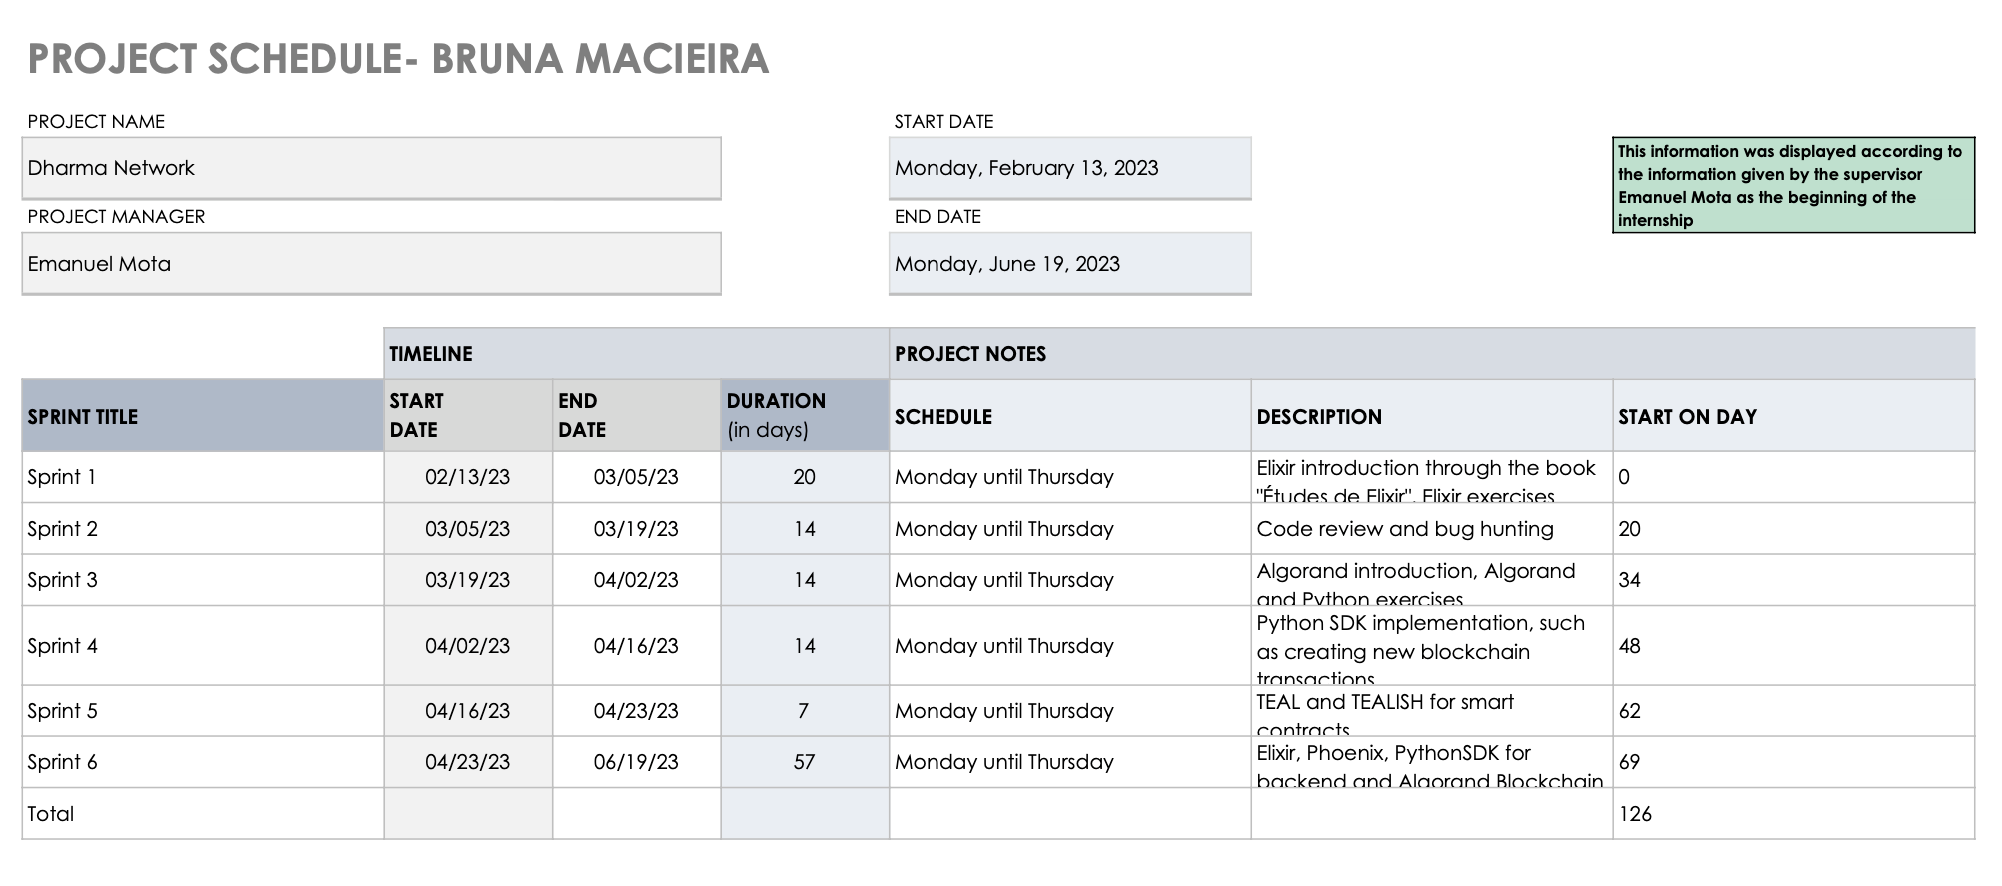
\includegraphics[scale=0.4]{Documentation/figures/sup_sch.png}  % largura percentual
	\caption{Intern's Initial Schedule}
	\label{sup_sch}
\end{figure}

 \begin{figure}[htbp]
	\centering
	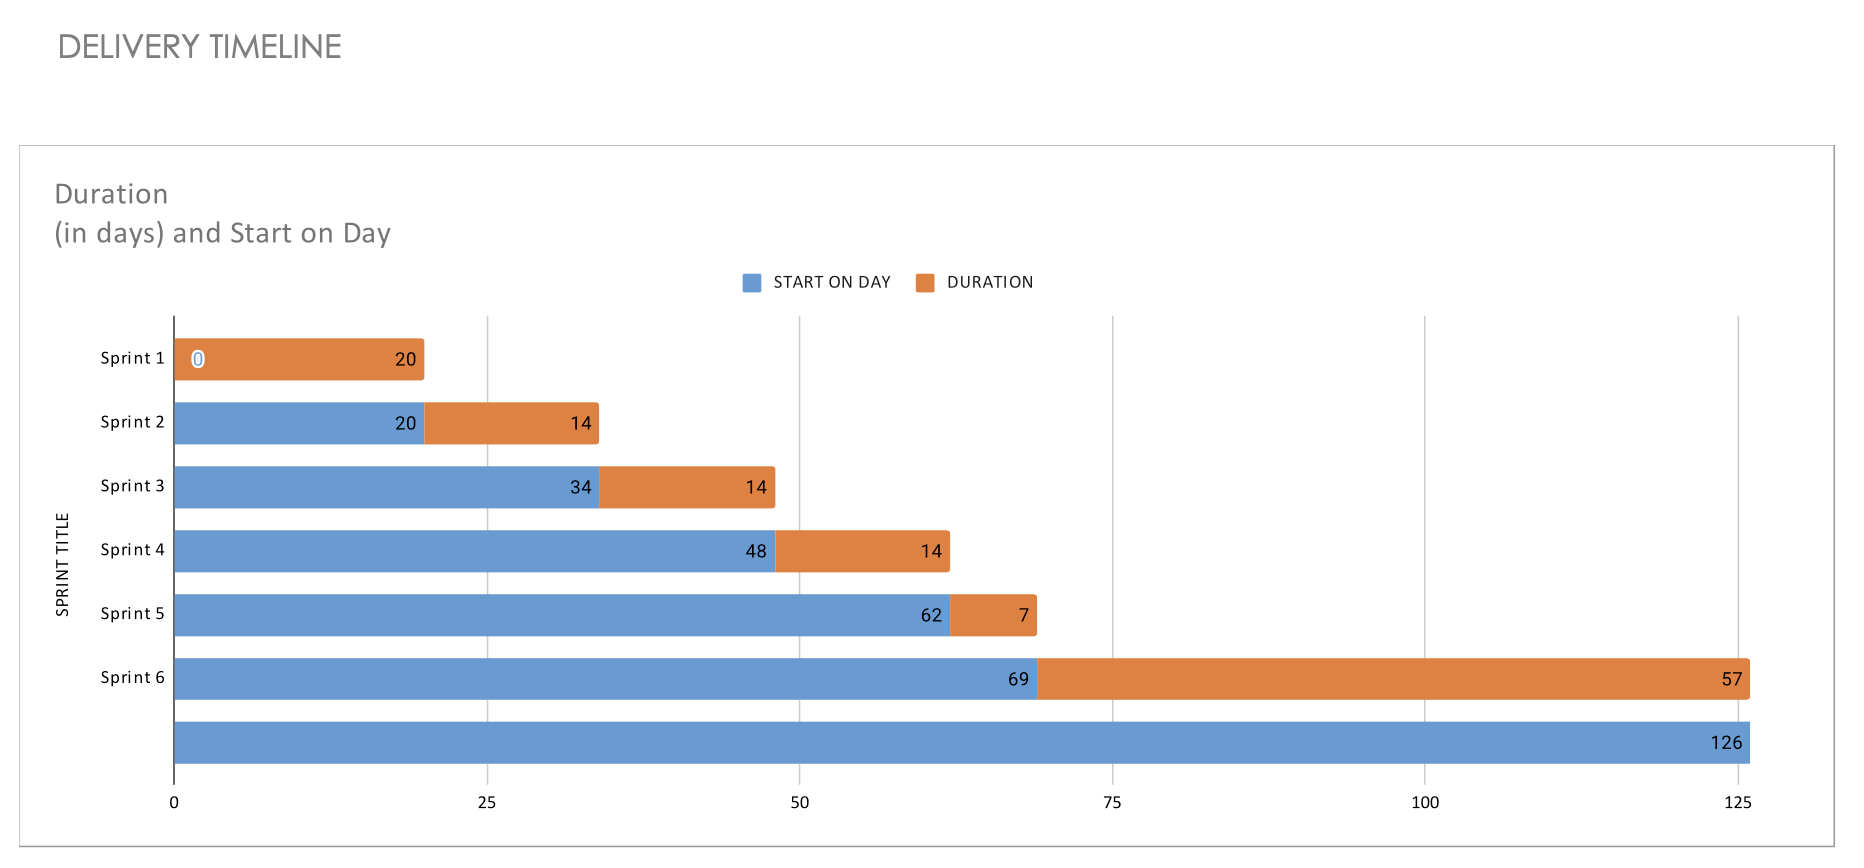
\includegraphics[scale=0.4]{Documentation/figures/sup_days.png}  % largura percentual
	\caption{Intern's Initial Sprint Distribution}
	\label{sup_days}
\end{figure}


However, due to the shortage of professionals working for Dharma Network and the need to advance the project, more experienced workers of the company developed the blockchain code, such as Smart Contracts and others.\newline

As a result, the project was developed according to the following guidelines on figures \ref{act_sch} and \ref{act_days}:\newline

 \begin{figure}[htbp]
	\centering
	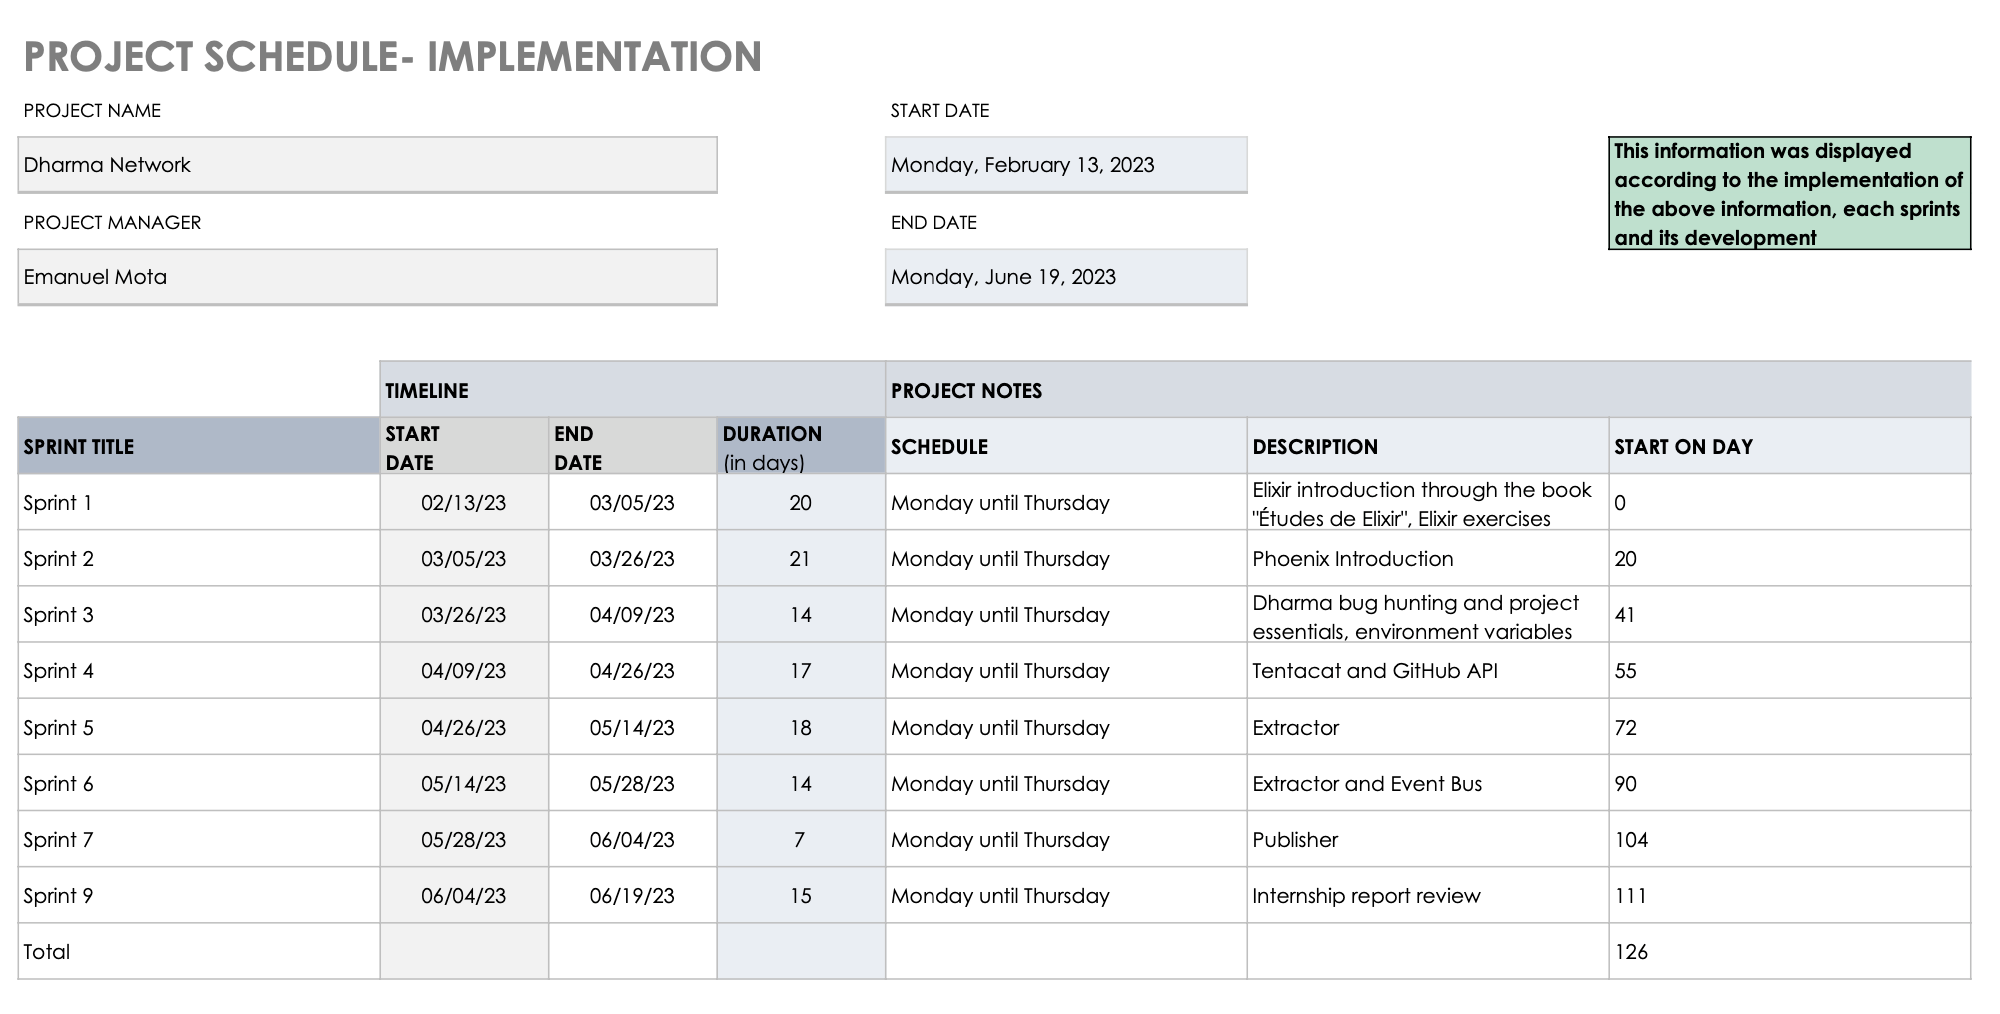
\includegraphics[scale=0.4]{Documentation/figures/act_sch.png}  % largura percentual
	\caption{Intern's Final Schedule}
	\label{act_sch}
\end{figure}

 \begin{figure}[htbp]
	\centering
	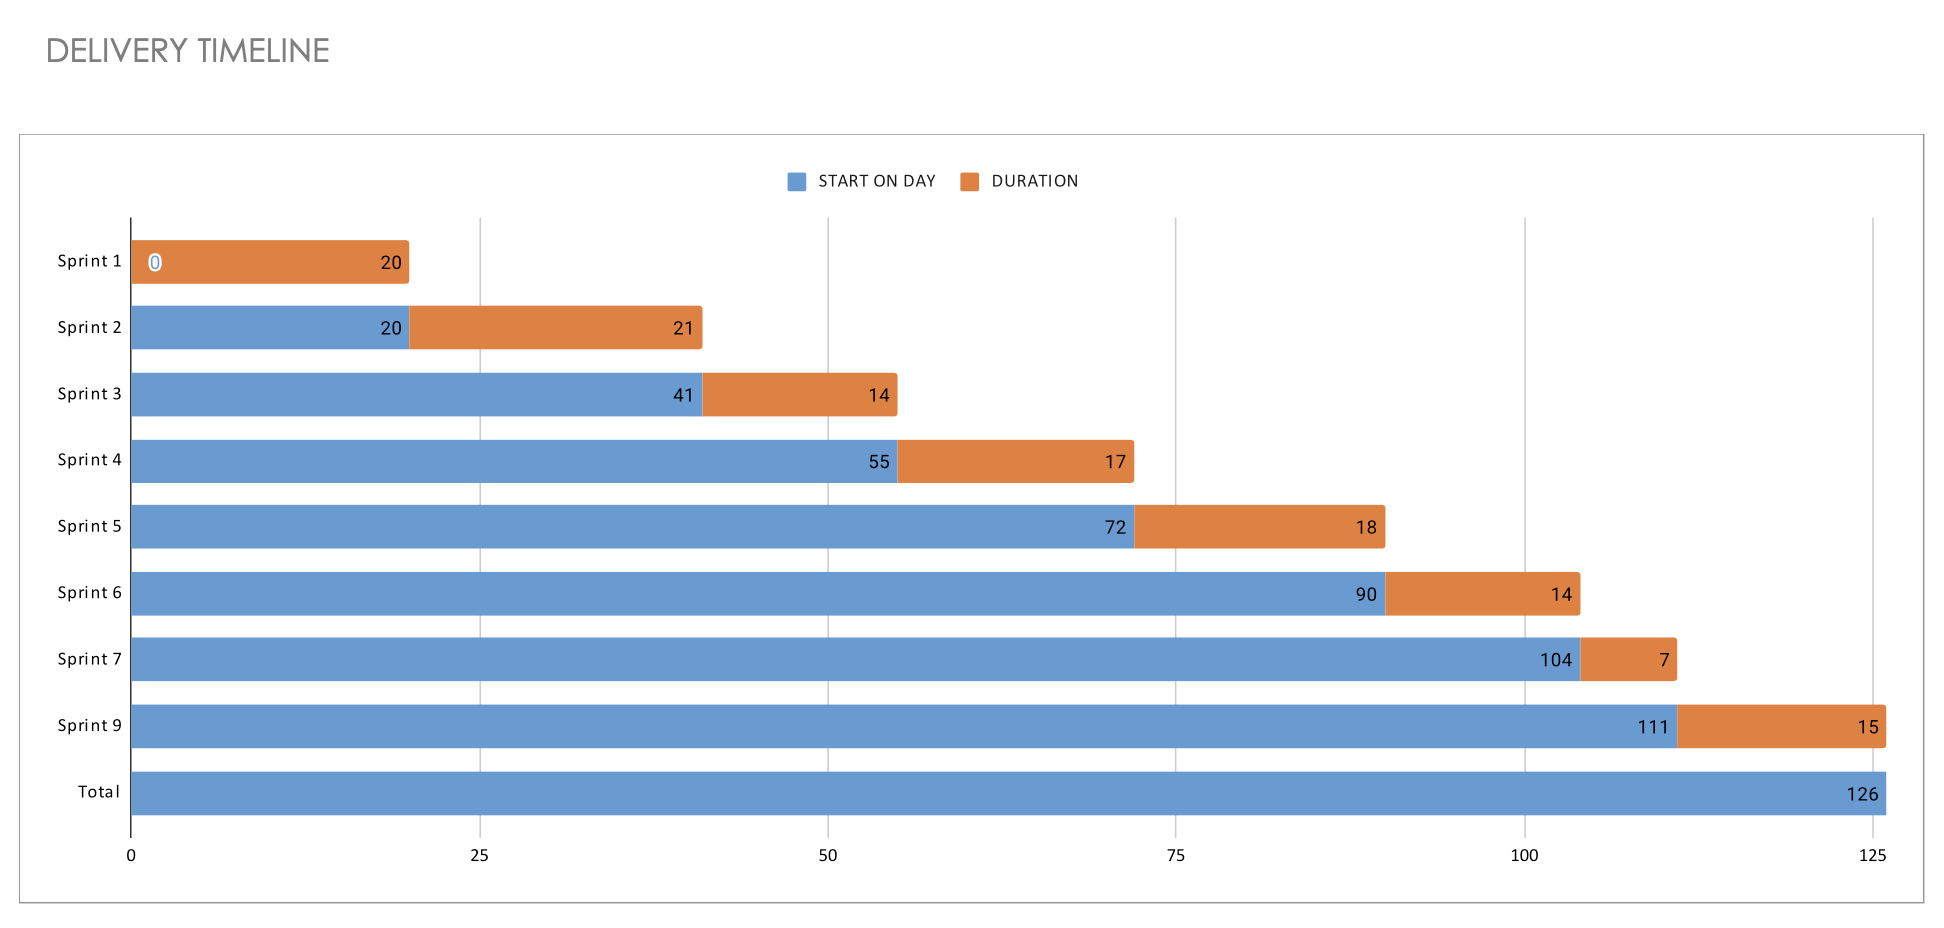
\includegraphics[scale=0.4]{Documentation/figures/act_days.png}  % largura percentual
	\caption{Intern's Final Sprint Distribution}
	\label{act_days}
\end{figure}

Figure \ref{sch} presents the hour counting of the internship and project distribution:


\begin{figure}[htbp]
	\centering
	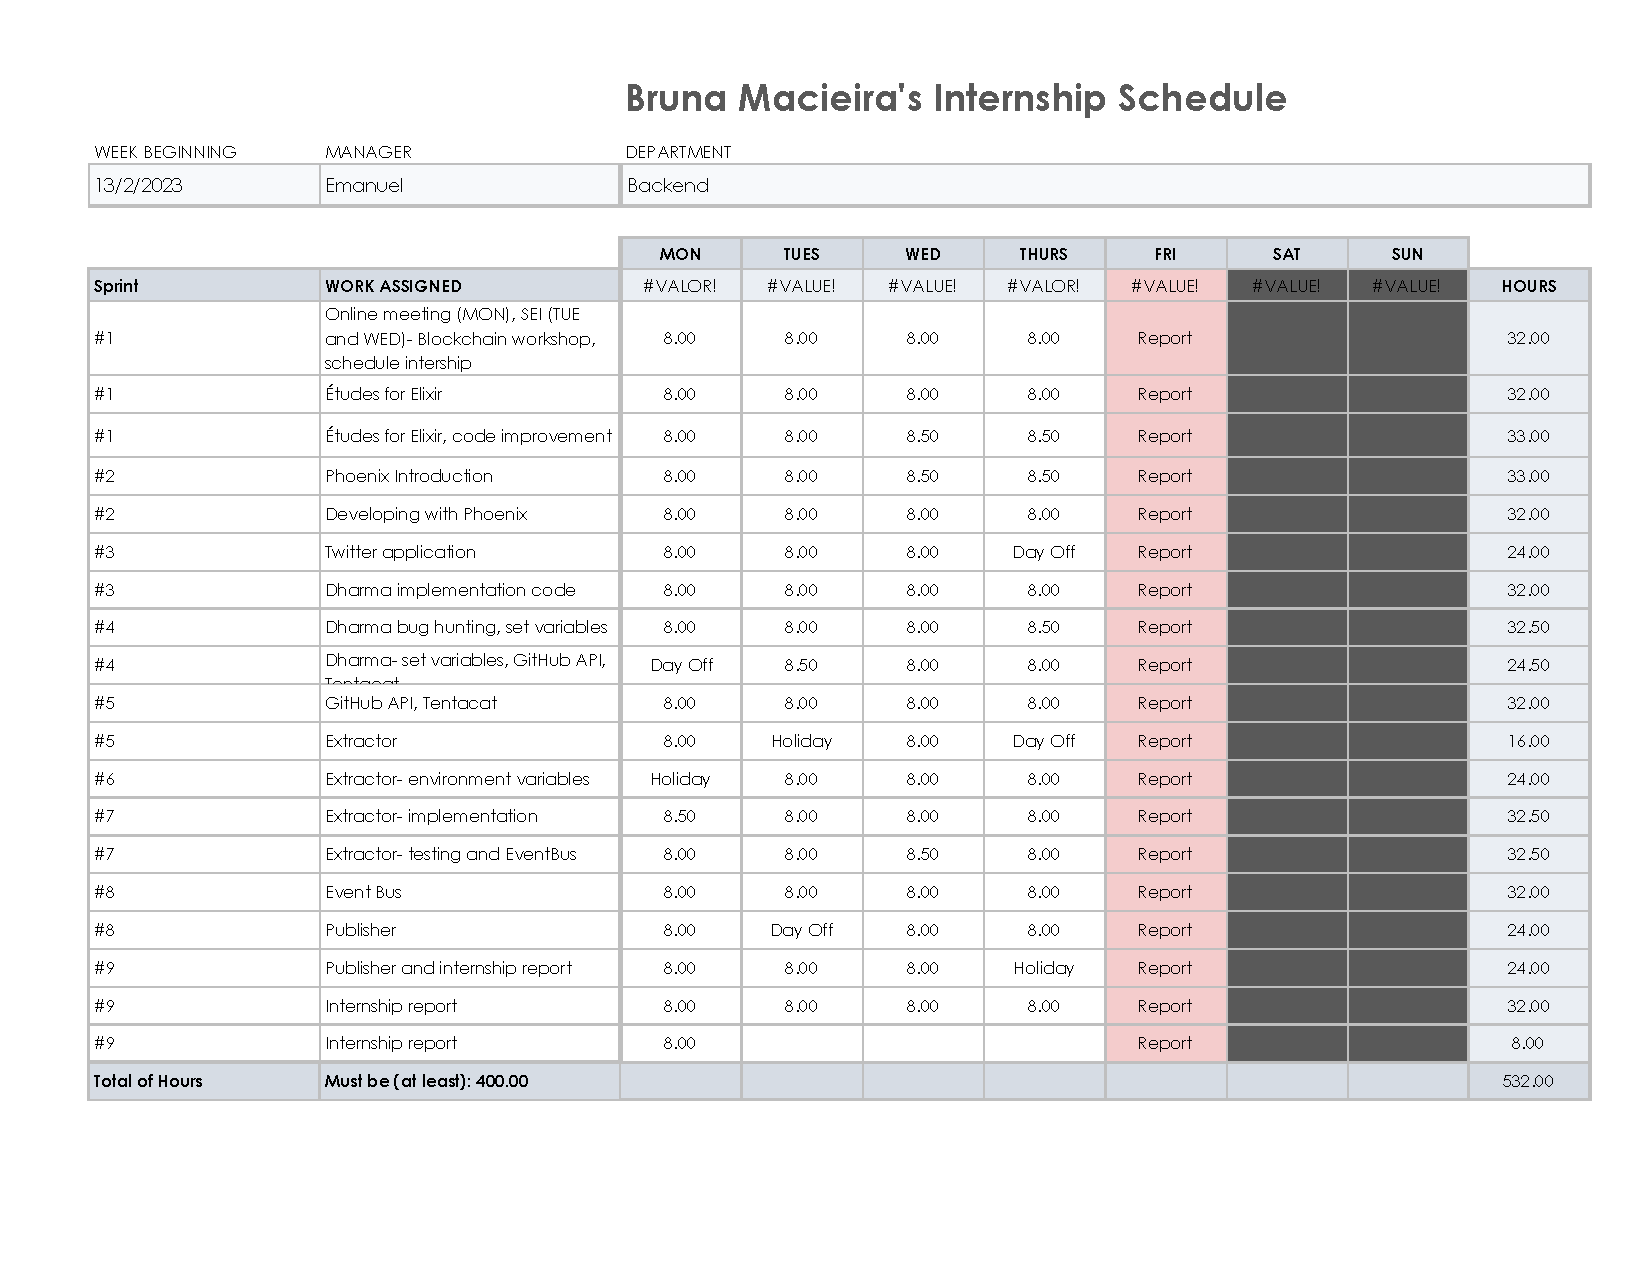
\includegraphics[scale=0.5]{Documentation/figures/Work_Hours - Work Schedule.pdf}  % largura percentual
	\caption{Intern's Internship Schedule and Hour Counting}
	\label{sch}
\end{figure}

\subsection{Final Analysis of the Project}

The blockchain components were built, but not by its original team. The backend components, however, were and continue to be developed by the original team.\newline

As far as the \textit{Proof of Real Work} of Dharma, it was implemented successfully, but it's not completed, since the publisher/consumer duo is not yet finished.\newline

The success of the Dharma Network project relies on continuous improvement and adaptation to evolving technological advancements, user demands and industry standards.